\section{Proposed NeST-Com Framework}
\subsection{Next-Scale Representation and Digital Frame}
We transmit $x\in[0,1]^{256\times256\times3}$ over complex AWGN,
\begin{equation}
 y=s+n,\quad n\sim\mathcal{CN}(0,\sigma^2 I_N),\quad
 \mathrm{SNR}=10\log_{10}(E_s/\sigma^2),
 \label{eq:channel}
\end{equation}
with $N=1024$ complex symbols per image and nominal $E_s=2$. The channel-use ratio to RGB samples is $1/192$. A 12-bit profile ID, CRC16, and terminated rate-1/2 convolutional code occupy 68 rotated-BPSK symbols $\{\pm(1+j)\}$. The remaining 956 symbols carry the LDPC-coded body. The paid profile identifies the actual endpoint and MCS.

The frozen VAR tokenizer produces ten residual token maps $q_s$, with side lengths $(1,2,3,4,5,6,8,10,13,16)$ and a 4096-entry codebook~\cite{var}. Let $L_s$ be the map size and $C_s$ its codebook lookup, resizing, and residual transform. The complete quantized latent is $f_q=\sum_s C_s(q_s)$. Image decoder $\Dc$ is adapted on 20\,000 ImageNet training images using continuous, fully quantized, and prefix-completion-interpolated latents, then fixed. NeST-Com uses null-class conditioning. Its frozen next-scale prior factorizes as
\begin{equation}
 p_\theta(q_s\mid q_{<s})=\prod_{i=1}^{L_s}p_\theta(q_{s,i}\mid q_{<s}),
 \label{eq:prior}
\end{equation}
providing the local cumulative distribution functions (CDFs) for arithmetic coding~\cite{arithmetic} at both ends of Fig.~\ref{fig:system}.

\begin{figure*}[t]
\centering
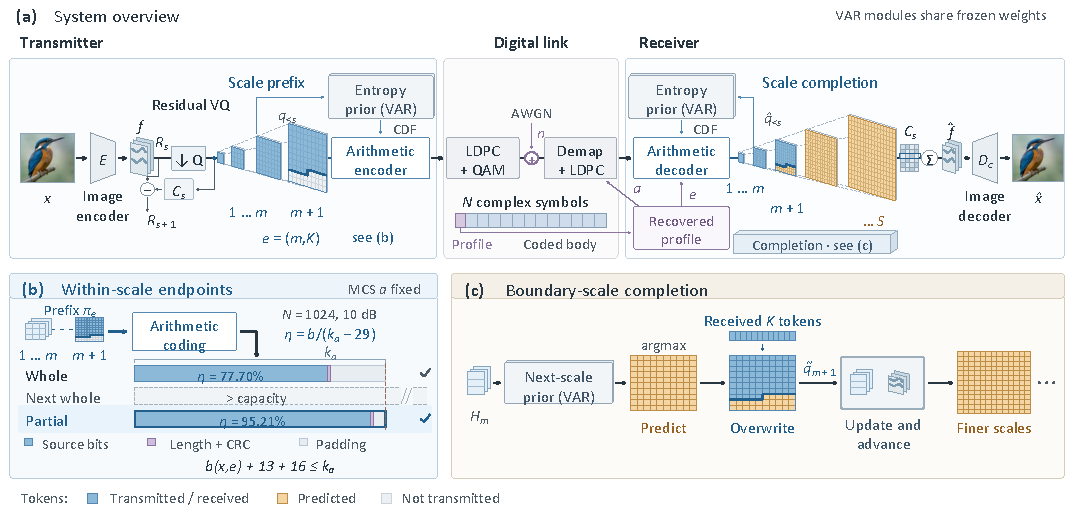
\includegraphics[width=\textwidth]{figure1.pdf}
\caption{NeST-Com. (a) A paid profile specifies endpoint $e$ and MCS $a$; TX/RX construct CDFs locally using the shared frozen VAR and their known coarse tokens. (b) Independently terminated prefixes, a 13-bit length field, and CRC16 fit the information capacity $k_a$. Bars illustrate common500 mean utilization at 10~dB, not an individual bitstream. (c) Received positions overwrite the predicted boundary map before residual accumulation and advancement to finer scales. $H_m$ denotes the prior state after scale $m$.}
\label{fig:system}
\end{figure*}

\subsection{Within-Scale Endpoints and Actual-Length Fitting}
An endpoint $e=(m,K)$ retains complete coarse maps and $K$ raster-ordered positions from the next map:
\begin{equation}
 \pi_e=(q_1,\ldots,q_m,q_{m+1,1:K}).
 \label{eq:prefix}
\end{equation}
WHOLE permits $K=0$. PARTIAL additionally uses
$K\in\{\lfloor L_{m+1}/4\rfloor,\lfloor L_{m+1}/2\rfloor,\lfloor3L_{m+1}/4\rfloor\}$ for $m=4,\ldots,9$; $(10,0)$ denotes the full representation.

For MCS $a=(M,r)$, the coded body has $n_a=956\log_2M$ bits and information length $k_a=\lfloor rn_a\rfloor$. With actual terminated arithmetic length $b(x,e)$,
\begin{equation}
 b(x,e)+29\leq k_a,\qquad \eta(x,e)=\frac{b(x,e)}{k_a-29}.
 \label{eq:budget}
\end{equation}
The 29 bits comprise the length field and CRC16; unused information positions are zero-padded before 5G NR LDPC coding, rate matching~\cite{nr}, and QAM. Thus $\eta$ measures entropy-stream capacity utilization.

Offline calibration selects an SNR-specific target endpoint, MCS, and ordered fallback chain using mean source/reconstruction DINOv2 cosine similarity~\cite{dinov2}. Online, the transmitter checks the target's terminated length and moves along that chain until~\eqref{eq:budget} holds, keeping the MCS fixed. The profile records the endpoint actually sent. This separates quality-based policy selection from per-image hard-budget fitting; an entropy estimate or a cut portion of a longer arithmetic stream is not the transmitted length.

\subsection{Prefix-Constrained Reconstruction}
Invalid profile CRC/catalogue, body CRC, declared length, known padding, or arithmetic parsing produces a fixed gray image. Otherwise, the receiver decodes the prefix using CDFs rebuilt from the complete coarse maps actually received. It predicts the boundary map by VAR argmax, then applies known-token overwrite~\cite{var}:
\begin{equation}
 \tilde q_{m+1,i}=\begin{cases}\hat q_{m+1,i},&i\leq K,\\q^{\mathrm{pred}}_{m+1,i},&i>K.\end{cases}
 \label{eq:overwrite}
\end{equation}
The merged map contributes directly to the residual latent and updates the prior state before finer-scale prediction. Complete received maps remain unchanged; subsequent maps are generated from this updated context. Reconstruction is
\begin{equation}
 \hat x=\Dc\!\left(\sum_{s=1}^{10}C_s(\tilde q_s)\right).
 \label{eq:reconstruction}
\end{equation}
At the final scale, overwrite changes the residual contribution without any subsequent propagation.
